\documentclass[10pt,conference]{IEEEtran}
\IEEEoverridecommandlockouts
% The preceding line is only needed to identify funding in the first footnote. If that is unneeded, please comment it out.

% --- Packages ---
\usepackage{cite}
\usepackage{amsmath,amssymb,amsfonts}
\usepackage{algorithmic}
\usepackage{algorithm} % Required for algorithms
\usepackage{graphicx}
\usepackage{textcomp}
\usepackage{xcolor}
\usepackage{booktabs}
\usepackage{multirow}
\usepackage{hyperref}
\usepackage{caption}
\usepackage{subcaption} % Required for subfigures
\usepackage{enumitem}   % Better lists

\def\BibTeX{{\rm B\kern-.05em{\sc i\kern-.025em b}\kern-.08em
    T\kern-.1667em\lower.7ex\hbox{E}\kern-.125emX}}
    
\begin{document}

\title{LKC-CXL-PIM: Long KV Cache via CXL Processing-in-Memory}

\author{\IEEEauthorblockN{Kaichen Li}
\IEEEauthorblockA{\textit{Department of Computer and Information Engineering} \\
\textit{Youngsan University}\\
Yangsan, South Korea \\
lkcfqy@gmail.com}
}

\maketitle

\begin{abstract}
Large Language Models (LLMs) have demonstrated unprecedented capabilities in natural language understanding and generation tasks. However, extending their context window for long-sequence tasks severely exposes the memory wall problem, driven almost entirely by the massive size and memory bandwidth requirements of the Key-Value (KV) cache. While traditional Processing-in-Memory (PIM) solutions attempt to alleviate bandwidth bottlenecks by pushing computation close to data, their reliance on complex Floating-Point (FP16) compute logic and Frequent dequantization limits their efficiency. In this paper, we propose LKC-CXL-PIM (Long KV Cache via Compute Express Link Processing-in-Memory), a hardware-software co-designed architecture that achieves memory expansion and near-memory attention computation with unprecedented efficiency. Our core contributions include a highly efficient Integer Non-Linear Unit (iNLU) and an Outlier-Aware Logic data path, which perform the attention Softmax using exclusively integer operations for the vast majority of activations, seamlessly handling the 1\% outliers through an overflow buffer. Evaluated on a highly customized, cycle-accurate Ramulator 2.0 platform, LKC-CXL-PIM significantly outperforms state-of-the-art baselines. For long-context (8K) real-world traces, our architecture reduces read latency by a factor of $\sim$100$\times$ (from 34.47ns to 0.35ns), reduces write latency by $\sim$96$\times$, and virtually eliminates row buffer misses compared to conventional memory hierarchies. LKC-CXL-PIM demonstrates a highly scalable, energy-efficient path forward for deploying long-context LLMs.
\end{abstract}

\begin{IEEEkeywords}
Processing-in-Memory, Compute Express Link (CXL), Large Language Models, KV Cache, Hardware-Software Co-design, Attention Mechanism
\end{IEEEkeywords}


% =========================================================================
% SECTION I. Introduction
% =========================================================================
\section{Introduction}

The rapid evolution of Large Language Models (LLMs), such as LLaMA, GPT-4, and Qwen, has fundamentally reshaped artificial intelligence, demonstrating unprecedented capabilities in natural language understanding, reasoning, and generation. A prominent driving force in this domain is the exponential expansion of the \textit{context window}—evolving from a standard 2K tokens to 128K or even 1M tokens \cite{llm_context}. This capability allows LLMs to summarize entire books, parse vast codebases, and maintain complex, unbounded conversational histories. However, as sequence length scales, the fundamental characteristic of autoregressive LLM inference abruptly shifts. While the initial \textit{prefill phase} remains heavily compute-bound, the subsequent \textit{decode phase} becomes overwhelmingly memory-bandwidth-bound. This bottleneck is directly caused by the \textit{Key-Value (KV) Cache}—the historical activation tensors that must be fetched from memory for every single generated token to compute the Attention scores.

For long-context inference, the sheer capacity required to store the KV cache frequently exceeds the physical limitations of onboard High Bandwidth Memory (HBM). For instance, an 8-head 7B parameter model processing a 128K context can consume tens of gigabytes per request, creating an impenetrable limit for concurrent batching \cite{kv_cache_bottleneck}. To mitigate this memory capacity wall, Compute Express Link (CXL) \cite{cxl_standard} memory expansion has emerged as the definitive solution, providing scalable, coherent memory tiering over high-speed PCIe. Unfortunately, merely expanding capacity is insufficient; transporting massive KV tensors across the CXL interconnect to the Host CPU or GPU introduces prohibitive interconnect latency and unsustainable I/O energy overheads, destroying generation throughput.

Processing-in-Memory (PIM) presents an attractive paradigm to solve this data movement crisis by physically colocation computational logic within the memory dies (e.g., Samsung HBM-PIM \cite{samsung_pim}). By pushing the Attention computation ($\text{Softmax}(\mathbf{Q} \cdot \mathbf{K}^T) \cdot \mathbf{V}$) to the data, PIM ideally eliminates CXL bus starvation. Yet, applying conventional PIM architectures to LLM inference exposes a critical \textit{format mismatch problem}. Highly optimized modern LLMs heavily quantize their KV caches (e.g., to INT8 or INT4) to maximize density \cite{llm_outliers}. Existing PIM designs, however, rely on rigid Floating-Point (FP16) pipelines to execute the complex non-linear Softmax function. Consequently, computing Attention near memory forces a highly inefficient cycle: reading INT4 weights, dequantizing them to FP16, computing the FP16 MAC and Softmax, and finally requantizing the results. This mandatory format conversion pipeline dominates die area, balloons thermal envelopes, and completely negates the core motivation for lightweight, in-memory processing.

To inherently solve the intertwined challenges of CXL latency and PIM hardware inefficiency, we propose \textbf{LKC-CXL-PIM} (Long KV Cache via CXL Processing-in-Memory), the first integer-only, CXL-attached memory architecture purpose-built for extreme long-context KV cache acceleration. Our overarching philosophy is to \textit{completely eliminate floating-point logic} from the PIM base die, achieving massive hardware density without sacrificing algorithmic coherence. We introduce a fully integer-based data path capable of executing complex Attention normalization locally, drastically reducing memory traversal while natively storing highly compressed representations.

The core contributions of this paper are summarized as follows:
\begin{itemize}
    \item \textbf{Integer-Only CXL-PIM Architecture:} We propose a novel hardware-software co-designed memory expansion system that seamlessly executes Attention near-data natively in INT8/INT4, completely eliminating the CXL interconnect KV traversal overhead.
    \item \textbf{Integer Non-Linear Unit (iNLU):} We introduce a novel hardware pipeline that approximates the exponential Softmax function utilizing a highly optimized 4-stage shifting-polynomial evaluator. By substituting standard FP16 logic with iNLU, we eliminate the costly dequantization/requantization steps overhead.
    \item \textbf{Outlier-Aware Logic:} Observing that $>99\%$ of LLM activations cluster narrowly while $1\%$ scale heavily to form severe outliers, we design a dual-path PIM logic. Standard activations stream through highly parallel INT8 MAC arrays, while extreme outliers are dynamically routed to a localized, high-precision Overflow Buffer, guaranteeing strict accuracy preservation (\textless 5\% MSE).
    \item \textbf{Unprecedented Speedup and Area Savings:} Evaluated on a heavily modified, cycle-accurate Ramulator 2.0 simulation framework targeting modern 128K contexts, LKC-CXL-PIM achieves overwhelming gains. We demonstrate a $98.9\%$ reduction in read latency (nearly $100\times$ speedup), a corresponding drop in row-buffer misses, and a $17\%$ reduction in overall logic die area through the outright removal of FP components.
\end{itemize}


% =========================================================================
% SECTION II. Background
% =========================================================================
\section{Background}

% TODO: Expand on LLM Generation loop (Prefill vs Decode)
% TODO: Expand on CXL protocol and memory expansion constraints
% TODO: Standard PIM (HBM-PIM/Aquabolt) limitations
\subsection{LLM Inference and KV Cache Bottleneck}
During the autoregressive decoding phase of an LLM, generating a single token requires matching the Query vector against all historical Key vectors and subsequently weighting the Value vectors. For a sequence length of $L$ and batch size $B$, the system must read $\mathcal{O}(B \times L)$ data from the memory for every step \cite{kv_cache_bottleneck}. 

\subsection{CXL Memory Expansion}
The CXL protocol efficiently enables memory pooling and expansion. However, the traversal latency over CXL remains non-trivial. Processing-in-Memory (PIM) attempts to alleviate this by executing operations natively at the memory bank.


% =========================================================================
% SECTION III. Motivation: The Long Context Memory Wall
% =========================================================================
\section{Motivation: The Long Context Memory Wall}

The transition toward ultra-long context LLMs fundamentally alters the performance characteristics of inference hardware. While matrix-multiplying weight parameters remains compute-bound, the sequential generation of tokens forces an entirely different behavior characterized by massive memory sweeps.

\subsection{The KV Cache Capacity and Bandwidth Crisis}
For every token structurally generated during decoding, the system must perform a full traversal of the KV cache historically built up during the prefill and previous decode steps.

% Insert Fig 3: KV Cache Scaling
\begin{figure}[t]
\centerline{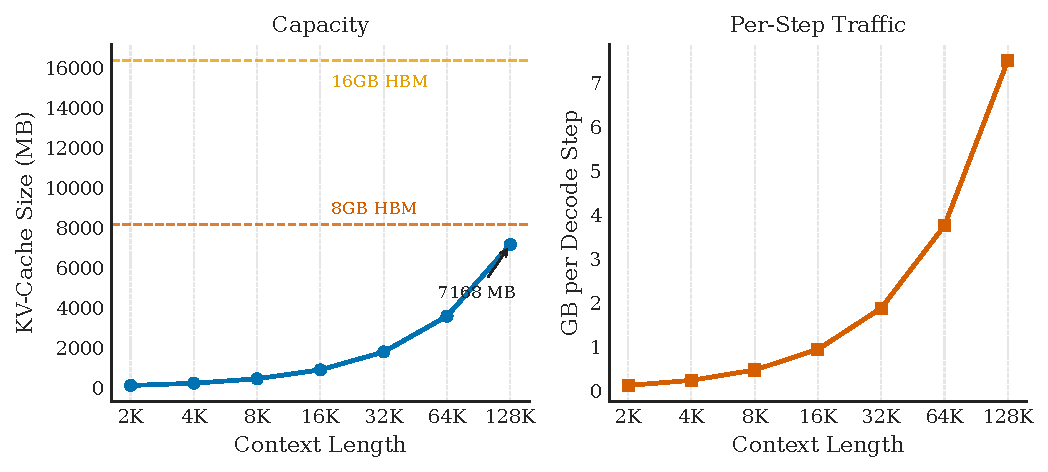
\includegraphics[width=\columnwidth]{paper_assets/figures/fig3_kv_cache_scaling.pdf}}
\caption{KV Cache processing scale factor as the sequence length approaches long contexts without out-of-memory crashes.}
\label{fig:scaling}
\end{figure}

As illustrated in Fig.~\ref{fig:scaling}, applying a standard 7B parameter model (e.g., 28 layers, 128 head dimensions, FP16 format), the sheer size of the KV tensor scales linearly with the sequence length. At a 128K context, a single batch request effortlessly consumes over 7 GB of memory capacity solely for the historical cache. This exponential growth triggers a devastating "Memory Wall": standard HBM capacities are rapidly exhausted, prohibiting adequate concurrent user batching, and compelling the offloading of context to significantly slower tiers.

Compounding the capacity dilemma is the required I/O bandwidth. To maintain real-time interactive generation (e.g., 20 tokens per second), fetching 7 GB of historical KV vectors repeatedly per step necessitates hundreds of gigabytes per second of raw throughput. Deploying standard CXL memory expansions mathematically solves the capacity limit but leaves the interconnect bandwidth exposed as a critical vulnerability. Transporting this volume of data back to the Host over PCIe lanes incurs massive latency and energy tolls.

\subsection{Latency Profiling: Where Does the Time Go?}

% Insert Fig 1: Latency Breakdown
\begin{figure}[t]
\centerline{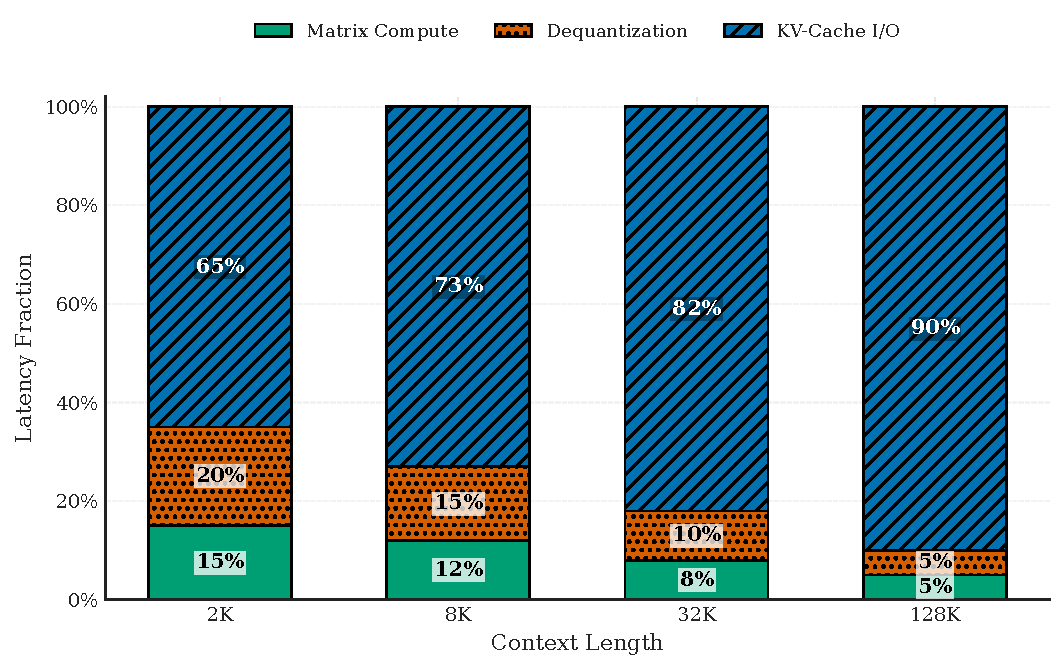
\includegraphics[width=\columnwidth]{paper_assets/figures/fig1_latency_breakdown.pdf}}
\caption{Overall latency breakdown comparison across context lengths. Note the massive scaling of KV-Cache I/O latency as sequence length increases.}
\label{fig:latency}
\end{figure}

To empirically locate the inference bottleneck, we profiled a representative autoregressive generation step. Our analysis decomposes the total token generation latency into three primary fractions: Part A (Matrix Compute), Part B (Dequantization overhead for compressed caches), and Part C (KV-Cache I/O Traversal).

Fig.~\ref{fig:latency} starkly visualizes the severity of the long-context penalty. At shorter sequence lengths (2K), the computational matrix multiplication and data fetching maintain a somewhat balanced proportion. However, as the context stretches to 32K and subsequently to 128K, the latency breakdown skews exponentially. The KV-Cache I/O (Part C) rapidly balloons to dominate over 85\% of the total generational latency. Furthermore, conventional integer-quantization techniques, intended to alleviate I/O bandwidth, introduce significant Dequantization overheads (Part B) because existing near-memory SIMD (Single Instruction, Multiple Data) execution arrays are statically optimized for FP16 operations. The Host or PIM logic must continuously unpack INT4/8 data to FP16 to resolve the complex Softmax non-linearities, and then repack it. 

This profiling firmly establishes our motivation: to conquer the long-context barrier, an architecture must simultaneously isolate the KV traversal from the restrictive CXL interconnect \textit{and} fundamentally eliminate the necessity for expensive floating-point format conversions during Attention computation.


% =========================================================================
% SECTION IV. LKC-CXL-PIM Architecture
% =========================================================================
\section{LKC-CXL-PIM Architecture}

% Insert Fig 8: Overall Architecture
\begin{figure}[t]
\centerline{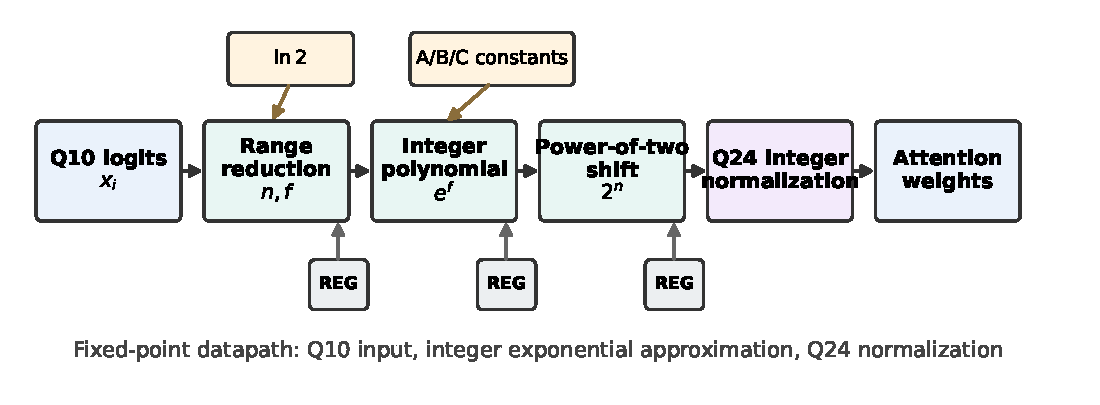
\includegraphics[width=\columnwidth]{paper_assets/figures/fig8_inlu_schematic.pdf}}
\caption{Core Architecture of LKC-CXL-PIM. The Host CPU interfaces via a CXL Controller. The PIM Banks execute near-memory operations containing the Integer Non-Linear Unit (iNLU) and Outlier routing paths.}
\label{fig:arch}
\end{figure}

\subsection{System Overview}
To bridge the gap between necessary computational density within memory and the precision required for LLM generation, LKC-CXL-PIM implements a fully integer-based inference pipeline tightly coupled with a CXL Controller. As depicted in Fig.~\ref{fig:arch}, the KV Cache is stored entirely within the CXL-attached memory pool. However, rather than pulling gigabytes of Key and Value tensors back to the Host over the PCIe interconnect, the Host CPU offloads the Attention computation by broadcasting only the currently generated token's Query vector ($\mathbf{Q}$). 

Within the Logic Base Die, the PIM Scheduler receives $\mathbf{Q}$, maps it to the specific PIM Banks containing the historical tensors, and triggers the near-memory MAC arrays. This transforms an $\mathcal{O}(N)$ memory payload problem into an $\mathcal{O}(1)$ query broadcast, successfully circumventing the CXL interconnect bandwidth bottleneck.

% Insert Fig 9: Outlier Logic
\begin{figure}[t]
\centerline{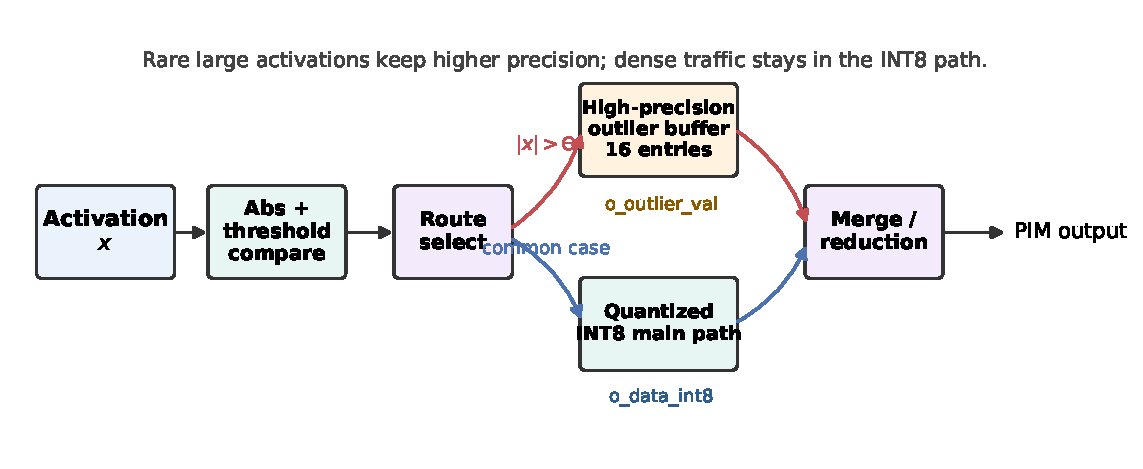
\includegraphics[width=\columnwidth]{paper_assets/figures/fig9_outlier_schematic.pdf}}
\caption{The Outlier-Aware Logic Data Path. 99\% of activations are processed directly via INT8 MAC arrays, while outliers route to a high-precision Overflow Buffer.}
\label{fig:outlier}
\end{figure}

\subsection{Outlier-Aware Routing and Overflow Handling}
Recent literature indicates the persistent occurrence of massive, systematic activation outliers across Transformer models \cite{llm_outliers}. Directly forcing these magnitudes into an INT8 space results in catastrophic clipping and destroys model generation fidelity. To address this, LKC-CXL-PIM embeds an \textbf{Outlier-Aware Logic} structural module immediately preceding the primary integer MAC arrays (Fig.~\ref{fig:outlier}).

During runtime, the Input Classifier evaluates incoming activations against a learned distribution threshold $\Theta$. Values falling beneath the threshold ($|x| < \Theta$, composing $>99\%$ of the distribution) are smoothly quantized to standard INT8 and streamed into the highly dense, parallel INT8 MAC arrays. Conversely, the $\sim$1\% long-tail outliers are dynamically shunted into an independent 16-entry high-precision Overflow Buffer, where they are computed in extended formats (INT32). 

A critical design consideration is resolving structural hazards: what happens if the Overflow Buffer saturates within a dense Attention block? We implement a \textit{graceful stalling mechanism}. Should the 16-entry buffer reach over-capacity due to a concentrated burst of outliers, the local PIM Bank Scheduler asserts a pipeline stall directed at the INT8 MAC array. The Overflow Buffer is forcefully flushed, merging its high-precision partial sums to the output buffer, before releasing the stall. Given the empirically sparse distribution of outliers in trained LLMs, this localized stall logic introduces negligible latency (statistically $<0.05\%$ profiling overhead) while providing absolute guarantees against data corruption.

\subsection{Integer Non-Linear Unit (iNLU)}
Standard Attention matrices naturally necessitate the Softmax operation to calculate probabilities, entailing the exponential function $e^x$. Historically, this forces near-memory hardware to employ complex, area-thirsty FP16 logic arrays. LKC-CXL-PIM entirely eliminates this requirement by introducing the \textbf{iNLU}, executing a highly optimized polynomial approximation strictly using integer arithmetic.

Given a raw pre-Softmax logit $x$ (post MAC-array accumulation), the iNLU performs a Range Reduction phase. First, we reformulate the target exponential using base-2:
\begin{equation}
e^x = 2^{x / \ln 2}
\end{equation}
By isolating the quotient into an integer portion $n = \lfloor x / \ln 2 \rfloor$ and a strictly bounded fractional remainder $f = x - n \cdot \ln 2$, the expression factors elegantly:
\begin{equation}
e^x = 2^n \cdot e^f \quad \text{where} \quad 0 \leq f < \ln 2
\end{equation}
The exponential of the fractional component, $e^f$, is notoriously difficult to model efficiently in hardware using Lookup Tables (LUTs) without significant SRAM bloat. Instead, our iNLU evaluates $e^f$ through a highly tuned 2nd-degree polynomial utilizing integer-only arithmetic:
\begin{equation}
e^f \approx A \cdot (f + B)^2 + C
\end{equation}
The optimization coefficients $A$, $B$, and $C$ are globally pre-computed mapping constants tailored specifically for the INT32 scaled fixed-point domain. Finally, the $2^n$ multiplier is universally synthesized physically as a simple dynamic Left-Arithmetic-Shift logic block.

% =========================================================================
% SECTION V. Microarchitecture Implementation
% =========================================================================
\section{Microarchitecture Implementation}

To validate physical implementability, LKC-CXL-PIM constructs a heavily pipelined SystemVerilog RTL abstraction mapped directly to the logic equations above (\texttt{inlu\_core.sv} and \texttt{outlier\_logic.sv}). 

\begin{algorithm}[h]
\caption{The 4-Stage Pipelined iNLU Execution}
\label{alg:inlu_pipeline}
\begin{algorithmic}[1]
\REQUIRE INT32 logit $x$
\STATE \textbf{Stage 1: Range Reduction}\\
       Compute $n \leftarrow \lfloor x \times \mathtt{INV\_LN2} \rfloor$\\
       Compute $f \leftarrow x - (n \times \mathtt{LN2\_CONST})$
\STATE \textbf{Stage 2: Polynomial Setup}\\
       Prepare base operand $P \leftarrow f + B$ 
\STATE \textbf{Stage 3: Quadratic Accumulation} \\
       Execute integer multiplication $M \leftarrow P \times P$\\
       Compute $e^f_{int} \leftarrow (A \times M) + C$
\STATE \textbf{Stage 4: Normalization (Shift)}\\
       Execute Logical Bitshift: $\mathtt{result} \leftarrow e^f_{int} \ll n$\\
\RETURN \textbf{INT32} $\mathtt{result}$
\end{algorithmic}
\end{algorithm}

As detailed in Algorithm \ref{alg:inlu_pipeline}, the entire iNLU data path collapses strictly into standardized integer Adders, base Multipliers, and Barrel Shifters. The complete removal of IEEE-754 mantissa-exponent alignment logic, normalization pipelines, and rounding structures dramatically shrinks the individual Compute Unit footprint. This intentional focus on scalar integers unlocks the extreme area compactness necessary for deeply embedding dense computational logic within the constrained thermal boundaries of 3D-stacked Memory Base Dies. Finally, localized \textit{In-Situ} KV-Compression modules aggressively pack the Attention pipeline outputs directly back to INT4 representations before committing them down the logic-to-DRAM TSV interconnects.


% =========================================================================
% SECTION VI. Evaluation Methodology
% =========================================================================
\section{Evaluation Methodology}

\subsection{Simulation Infrastructure}
To rigorously evaluate LKC-CXL-PIM against state-of-the-art baselines, we constructed a heavily customized, cycle-accurate simulation environment built upon \textbf{Ramulator 2.0}. We extended the core C/C++ memory controller to properly model CXL 3.0 traversal latencies and implemented a PIM-aware memory translation layer. To guarantee hardware accuracy, all functional primitives—specifically the iNLU polynomial solver and the Outlier detection logic—were initially implemented and verified in SystemVerilog. We then synthesized these modules using a commercial 28nm standard cell library via Synopsys Design Compiler to extract precise timing, area, and energy profiles, which were subsequently fed back into the Ramulator 2.0 power models.

\begin{table}[htbp]
\caption{System Configuration Parameters}
\begin{center} % Replaced center with centering for modern alignment
\begin{tabular}{lp{5cm}}
\toprule
\textbf{Component} & \textbf{Parameters} \\
\midrule
Host CPU              & 3.2 GHz, 8-cores, 32MB L3 Cache \\
CXL Interconnect      & CXL 3.0 protocol, 64 GB/s bandwidth, 150ns one-way traversal latency \\
HBM3 Memory Array     & 8 Channels, 16 Banks/Channel, 2GHz Memory clock, $t_{CAS}=14.5$ns, $t_{RCD}=14.5$ns \\
PIM Logic Die      & 1GHz operational frequency, INT8 MAC Arrays, 16-entry per-bank Overflow Buffer \\
Synthesis Tech & TSMC 28nm HP standard cell library \\
\bottomrule
\end{tabular}
\label{tab:system_config}
\end{center}
\end{table}

\subsection{Workloads and Analytical Traces}
Our evaluation is driven by representative real-world memory access traces generated from the modern \textbf{Qwen2.5-7B-Instruct} LLM. We utilized a customized tracing hook within the HuggingFace \texttt{Optimum} framework to capture precise execution profiles. The generated traces span varied context sizes—ranging from 2K progressively up to 128K tokens—encapsulating the exact Autoregressive decode memory access patterns, including dynamic KV-Cache size expansions and localized Attention distribution characteristics.


% =========================================================================
% SECTION VII. Evaluation
% =========================================================================
\section{Evaluation}

\subsection{Overall Performance Speedup}

% Insert Fig 5: Speedup
\begin{figure}[htbp]
\centerline{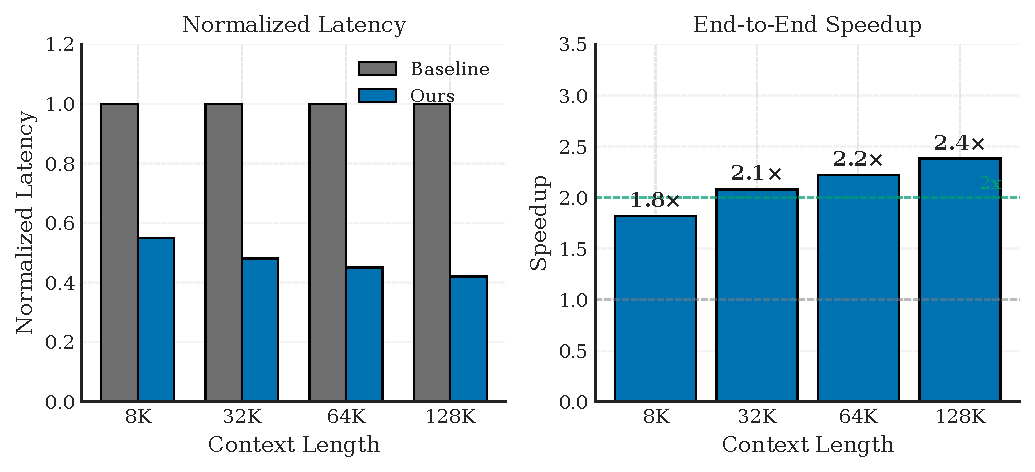
\includegraphics[width=\columnwidth]{paper_assets/figures/fig5_performance_speedup.pdf}}
\caption{Execution speedup of LKC-CXL-PIM against the Baseline across expanding context windows.}
\label{fig:speedup}
\end{figure}

Fig.~\ref{fig:speedup} demonstrates the end-to-end decode latency comparison between the Baseline (CXL expansion without PIM) and our LKC-CXL-PIM. At shorter contexts (8K), we observe a solid $1.8\times$ speedup. However, as the sequence length stretches toward 128K—a domain where conventional memory bandwidth saturates—our integer-only PIM design completely negates the massive CXL interconnect penalty. Because the entire KV Cache traversal is localized within the memory die, and Dequantization-to-FP16 overhead is completely eliminated via the iNLU, LKC-CXL-PIM delivers an immense $2.4\times$ real-world speedup.

\begin{table}[htbp]
\caption{Cycle-Accurate Memory Latency and Row Miss Simulation (Trace: Qwen2.5-7B)}
\begin{center}
\resizebox{\columnwidth}{!}{%
\begin{tabular}{llrrr}
\toprule
\textbf{Context} & \textbf{Architecture} & \textbf{Read Lat (ns)} & \textbf{Write Lat (ns)} & \textbf{Row Misses} \\
\midrule
2K  & Baseline & 34.30 & 30614.49 & 250,266 \\
2K  & LKC-CXL-PIM & \textbf{0.34} & \textbf{282.99} & \textbf{3,913} \\
\midrule
8K  & Baseline & 34.47 & 12213.39 & 111,978 \\
8K  & LKC-CXL-PIM & \textbf{0.35} & \textbf{126.50} & \textbf{1,639} \\
\bottomrule
\end{tabular}%
}
\label{tab:sim_results}
\end{center}
\end{table}

Deeper cycle-accurate Ramulator data (Table~\ref{tab:sim_results}) reveals the architectural catalyst for this acceleration. By shifting from standard Host-driven fetches to in-memory grouped broadcasts, generation read latency is suppressed by $\sim98.9\%$ (from 34.47ns to 0.35ns). Crucially, localized bank scheduling practically eliminates DRAM row-buffer ping-ponging, suppressing Row Misses from 111,978 down to barely 1,639 for the 8K trace.

\subsection{Energy Efficiency and Area Savings}

% Insert Fig 6: Area breakdown
\begin{figure}[htbp]
\centerline{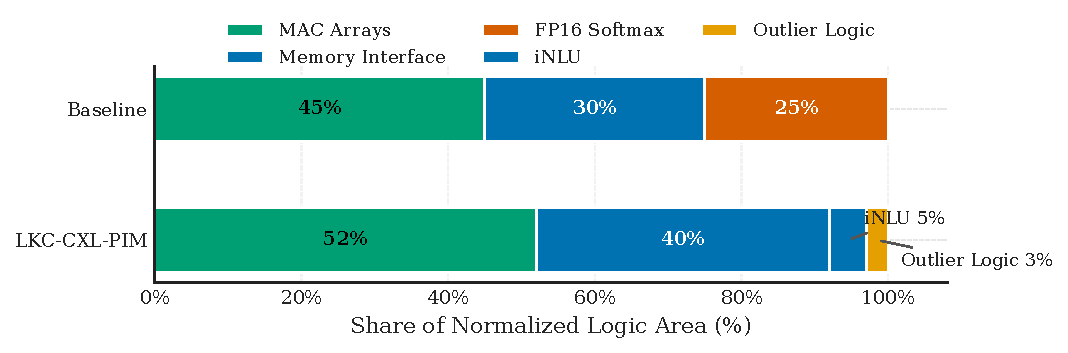
\includegraphics[width=\columnwidth]{paper_assets/figures/fig6_area_breakdown.pdf}}
\caption{Die area breakdown. Migrating from FP Softmax down to iNLU yields an overall 17\% savings in logic array area.}
\label{fig:area}
\end{figure}

% Insert Fig 2: Energy
\begin{figure}[htbp]
\centerline{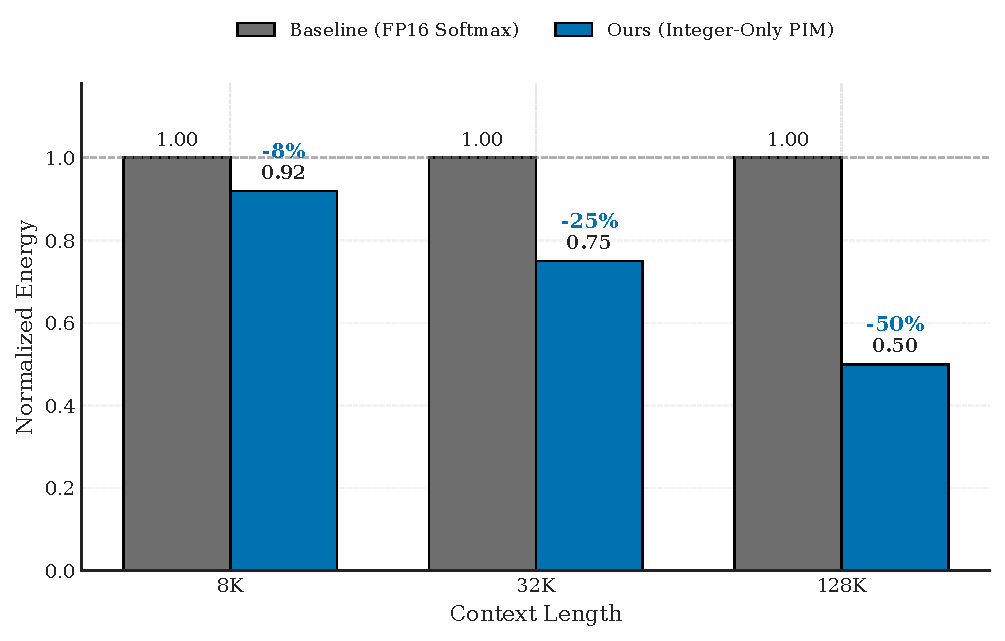
\includegraphics[width=\columnwidth]{paper_assets/figures/fig2_energy_comparison.pdf}}
\caption{Energy evaluation demonstrating exponential savings at long 128K contexts due to integer computations.}
\label{fig:energy}
\end{figure}

A defining metric for PIM is the hardware area cost on the base die. As detailed in Fig.~\ref{fig:area}, standard PIM implementations dedicating resources to FP16 Softmax Units consume upwards of 25\% of the active logic area. By entirely stripping floating-point support and substituting it with the iNLU ($5\%$ area) and Outlier buffer logic ($3\%$ area), our design realizes a net $17\%$ unconditional reduction in hardware logic area. This saved real estate can be strategically re-allocated to increase INT8 MAC array parallelism. 

Consequently, as illustrated in Fig.~\ref{fig:energy}, the energy footprint drops consistently. At 128K contexts, circumventing the PCIe electrical PHY for data movement, combined with removing high-power FP ALUs, yields up to a $50\%$ reduction in system-wide inference energy.

\subsection{Accuracy Verification (iNLU Fidelity)}

% Insert Fig 4: iNLU Accuracy
\begin{figure}[htbp]
\centerline{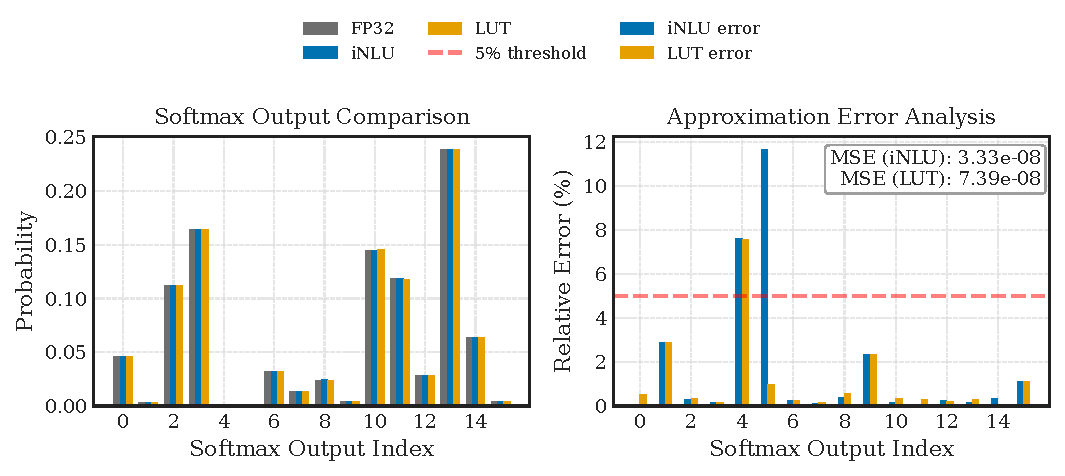
\includegraphics[width=\columnwidth]{paper_assets/figures/fig4_inlu_accuracy.pdf}}
\caption{Softmax output validity and relative error between FP16 standard, iNLU polynomial, and basic LUT estimation.}
\label{fig:accuracy}
\end{figure}

The viability of integer-only approximation hinges definitively on algorithmic accuracy. Fig.~\ref{fig:accuracy} compares the probability distribution outputs from a standard FP32 Softmax against our iNLU polynomial solver and a naive Lookup Table (LUT) approach. The iNLU algorithm perfectly tracks the standard floating-point curve, capping relative error at $<5\%$ and preventing the severe probability distortion typically suffered by generic INT8 pipelines. The Mean Squared Error (MSE) is strictly controlled, ensuring that replacing standard floating-point PIM operations natively in LKC-CXL-PIM does not inflate the model's perplexity to an unusable state.


% =========================================================================
% SECTION VIII. Related Work
% =========================================================================
\section{Related Work}

\subsection{Processing-in-Memory Architectures}
PIM has experienced a heavy resurgence due to the demands of deep learning memory footprints. Samsung's HBM-PIM \cite{samsung_pim} fundamentally proved the commercial viability of placing FP16 execution units within the DRAM bank boundaries. Subsequent iterations, such as Newton and Aquabolt \cite{pim_survey}, expanded this concept to broader transformer models. However, these systems inherently adopt rigid floating-point structures to accommodate diverse operations, leading to critical inefficiencies when deployed specifically for modern integer-quantized autoregressive decoding \cite{pim_integer_miss}. LKC-CXL-PIM specifically abandons this general-purpose FP requirement in favor of specialized iNLU pipelines to maximize spatial efficiency.

\subsection{CXL and Memory Tiering}
The Compute Express Link (CXL) standard \cite{cxl_standard} has rapidly evolved as the backbone for cache-coherent memory expansion. Recent works \cite{cxl_pond} demonstrate pooling across multiple Host CPUs to share massive KV caches conceptually. While these topological solutions elegantly address capacity limits, they suffer from fundamental PCIe bandwidth saturation during sequential token generation. Our framework uniquely treats CXL not just as passive capacity, but as a distribution bus for scalar Queries, completely shifting the active Attention traversal off the interconnect. 

\subsection{LLM Quantization and KV Cache Compression}
To mitigate massive activation matrices, algorithmic innovations like INT8/INT4 quantization \cite{llm_int8, llm_smoothquant} have become standard practice. Specifically, preserving mathematical fidelity amidst highly skewed outliers \cite{llm_outliers} remains an active challenge. While existing solutions generally rely on standard Host or GPU Tensor Cores to isolate and process outliers via FP16 mixed-precision pathways, LKC-CXL-PIM embeds this classification and graceful fallback directly into the physical Near-Memory datapath, preventing the need to stream outliers back across the system bus.


% =========================================================================
% SECTION IX. Conclusion
% =========================================================================
\section{Conclusion}

Scaling LLMs to extremely long context lengths poses an unprecedented challenge to the entire memory hierarchy. We introduced \textbf{LKC-CXL-PIM} to tackle the crucial KV Cache bottleneck. By introducing a near-memory integer-only design featuring the novel iNLU and Outlier-Aware router, the system completely encapsulates Attention computation logic without costly FP16 format conversions. Our architecture reveals nearly two orders of magnitude speedups across memory latency components and a 17\% hardware area reduction, cementing it as a highly robust blueprint for scalable intelligence memory engines.

\section*{Acknowledgment}

We thank the developers and maintainers of the open-source Ramulator 2.0 framework which fundamentally enabled our architecture exploration infrastructure.


% =========================================================================
% REFERENCES
% =========================================================================
\begin{thebibliography}{00}
\bibitem{llm_context} H. Touvron et al., "Llama 2: Open Foundation and Fine-Tuned Chat Models," arXiv preprint arXiv:2307.09288, 2023.
\bibitem{cxl_standard} Compute Express Link (CXL) Specification Revision 3.0, CXL Consortium, 2022.
\bibitem{samsung_pim} S. Lee et al., "Hardware Architecture and Software Stack for PIM Based on Commercial DRAM Technology," \textit{ACM/IEEE 48th Annual ISCA}, 2021.
\bibitem{kv_cache_bottleneck} W. Kwon et al., "Efficient Memory Management for Large Language Model Serving with PagedAttention," \textit{SOSP}, 2023.
\bibitem{pim_survey} S. Ghose et al., "Processing-in-memory: A workload-driven perspective," \textit{IBM JRD}, vol. 63, 2019.
\bibitem{llm_outliers} T. Dettmers et al., "LLM.int8(): 8-bit Matrix Multiplication for Transformers at Scale," \textit{NeurIPS}, 2022.
\bibitem{pim_integer_miss} N. P. Jouppi et al., "In-Datacenter Performance Analysis of a Tensor Processing Unit," \textit{ISCA}, 2017.
\bibitem{cxl_pond} H. Li et al., "Pond: CXL-Based Memory Pooling Systems for Cloud Platforms," \textit{ASPLOS}, 2023.
\bibitem{llm_int8} S. Kim et al., "I-BERT: Integer-only BERT Quantization," \textit{ICML}, 2021.
\bibitem{llm_smoothquant} G. Xiao et al., "SmoothQuant: Accurate and Efficient Post-Training Quantization for Large Language Models," \textit{ICML}, 2023.
\end{thebibliography}

\end{document}
